\chapter{Porting Tang}\label{porting-tang}

\section{Install dependencies}

update feeds
feeds install
make menuconfig
\newpage



to have an example created simple application in C for xinetd
\newpage

\section{Cross-compile Tang}

do not forget to add xinetd in Dependencies
\newpage

\subsection{Concealing http-parser}

without upstream patch not working tang
\newpage

\subsection{Mysterious José}

does makefiles support shell {a,b} thing???
\newpage

\section{Configure Tang with xinetd}

We need xinetd's socket activation for Tang to work.
\section{Socket activation with xinetd}

\begin{figure}[h]
    \centering
    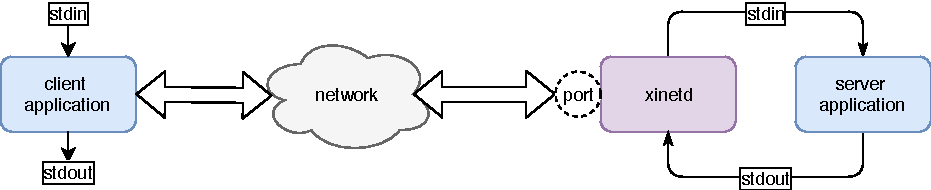
\includegraphics[scale=0.9]{figures/xinetd.pdf}
    \caption{xinetd socket activation}
    \label{fig_xinetd}
\end{figure}

there is no systemd for OpenWrt
need to configure socket activation because tang is not proggramed to use nor create its own sockets
\subsection{How }
\subsection{systemd}\label{systemd} % vymazat ako subsection
systemd is a suite of basic building blocks for a Linux system.
It provides a system and service manager that runs as PID 1 and starts the rest of the system.
systemd provides aggressive parallelization capabilities, uses socket and D-Bus activation for starting services,
 offers on-demand starting of daemons, keeps track of processes using Linux control groups, maintains mount and automount points,
 and implements an elaborate transactional dependency-based service control logic.
\todo{Why is systemd needed by tang}

/etc/services

xinetd configuration

\subsection{}


% root@A04-0315A:~# if [ -z "$(find /usr/share/tang/db/ -name "*.jw*" -maxdepth 1)" ]; then echo nic; else echo daco;fi
% daco
% root@A04-0315A:~# if [ -z "$(find /usr/share/tang/db/ -name "*.jwk" -maxdepth 1)" ]; then echo nic; else echo daco;fi
% daco
